%\chapter{Introduction}
\chapter{绪论}
\label{chapter:Introduction}
%\epigraph{Saving our planet, lifting people out of poverty, advancing economic growth... these are one and the same fight. We must connect the dots between climate change, water scarcity, energy shortages, global health, food security and women's empowerment. Solutions to one problem must be solutions for all.}{\textit{Ban Ki-moon}}

%This dissertation considers a way to solve the global problems of energy shortage and environment problem.

%\section{Research background and significance}
\section{研究背景及意义}
% 现有太阳能光热发电技术简析,提出太阳能梯级发电的背景及其意义。

% 能源和环境现状
%Renewables are now established around the world as mainstream sources of energy. Rapid growth, particularly in the power sector, is driven by several factors, including the improving cost-competitiveness of renewable technologies, dedicated policy initiatives, better access to financing, energy security and environmental concerns, growing demand for energy in developing and emerging economies, and the need for access to modern energy.
可再生能源在世界范围内已经成为主流能源。可再生能源,尤其是清洁电力的快速发展,受到诸多因素的推动,包括可再生能源技术成本的降低,政府专项政策的推动,融资渠道更加完善,能源安全和环境问题,发展中国家和新兴经济体对能源需求的不断增长,以及获得现代能源的需求。

% 太阳能光热发电现状
%Solar energy, which has the advantages of widely distribution, huge amount, inexhaustible and no pollution, has received much attention by many countries and been regarded as the best potential candidate of the fossil energy. The International Energy Agency projected in 2014 that under its ``high renewables'' scenario, by 2050, solar photovoltaics and concentrating solar thermal power would contribute about 16 and 11 percent, respectively, of the worldwide electricity consumption, and solar would be the world's largest source of electricity.~\cite{IEA2014}
太阳能因具有分布广泛,能量巨大,取之不竭,安全环保等优点,受到很多国家的关注,被认为是化石能源的最佳潜在替代者。国际能源机构预计,到2050年“大量应用可再生能源”的情景下,太阳能光伏发电量和太阳能光热发电量将分别占全球总用电量的16\%和11\%,太阳能将成为全球最大的电力来源\cite{IEA2014}。

%Concentrating solar thermal power generation is another form of power generation technology except solar photovoltaic power generation. Concentrating Solar Power (CSP) system uses mirrors to converge sunlight onto a receiver that absorbs the solar energy and transfer it to a heat transfer fluid (HTF) such as a synthetic oil, molten salt or air. The HTF then directly or indirectly used as the heat source in a power cycle.
%Compared to solar photovoltaic, solar thermal power is gaining more attention for its advantages as higher energy density, smooth power generation, good grid compatibility, easy to integrate with existing fossil power plant.
太阳能光热发电是除太阳能光伏发电之外的另一种太阳能发电技术。由于太阳能能量密度较低,为了提高可用的能量密度,太阳能光热发电通常采用聚光集热发电(CSP)的形式,使用反射镜将太阳光会聚到用于吸收太阳能的接收器上,产生热量并将其传递给合成油,熔融盐或空气等传热流体。然后,传热流体直接或间接地为动力循环系统提供热源。
与太阳能光伏发电相比,太阳能集热发电因其能量密度高,发电平稳,电网兼容性好,易于与现有火力发电厂集成等优点受到越来越多的关注。


% 文献1
%Concentrating solar power technologies use different mirror configurations to concentrate the sun's light energy onto a receiver and convert it into heat. The heat is collected for power generation or used as industrial process heat.
%There are three types of CSP technologies being commercially applied: parabolic trough, parabolic dish and power tower.
%Figure~\ref{fig:collectors} shows examples of the three types of CSP technologies.
太阳能光热发电技术使用不同种类的反射镜将太阳的光能会聚到接收器上并将其转换成热量。
现有三种已商业应用的CSP技术:太阳能槽式发电,太阳能碟式发电和太阳能塔式发电。这三种集热发电技术因其各自的反射镜类型而得名。
图\ref{fig:collectors}展示了这三种CSP技术的应用实例。
\begin{figure}[!ht]
\centering
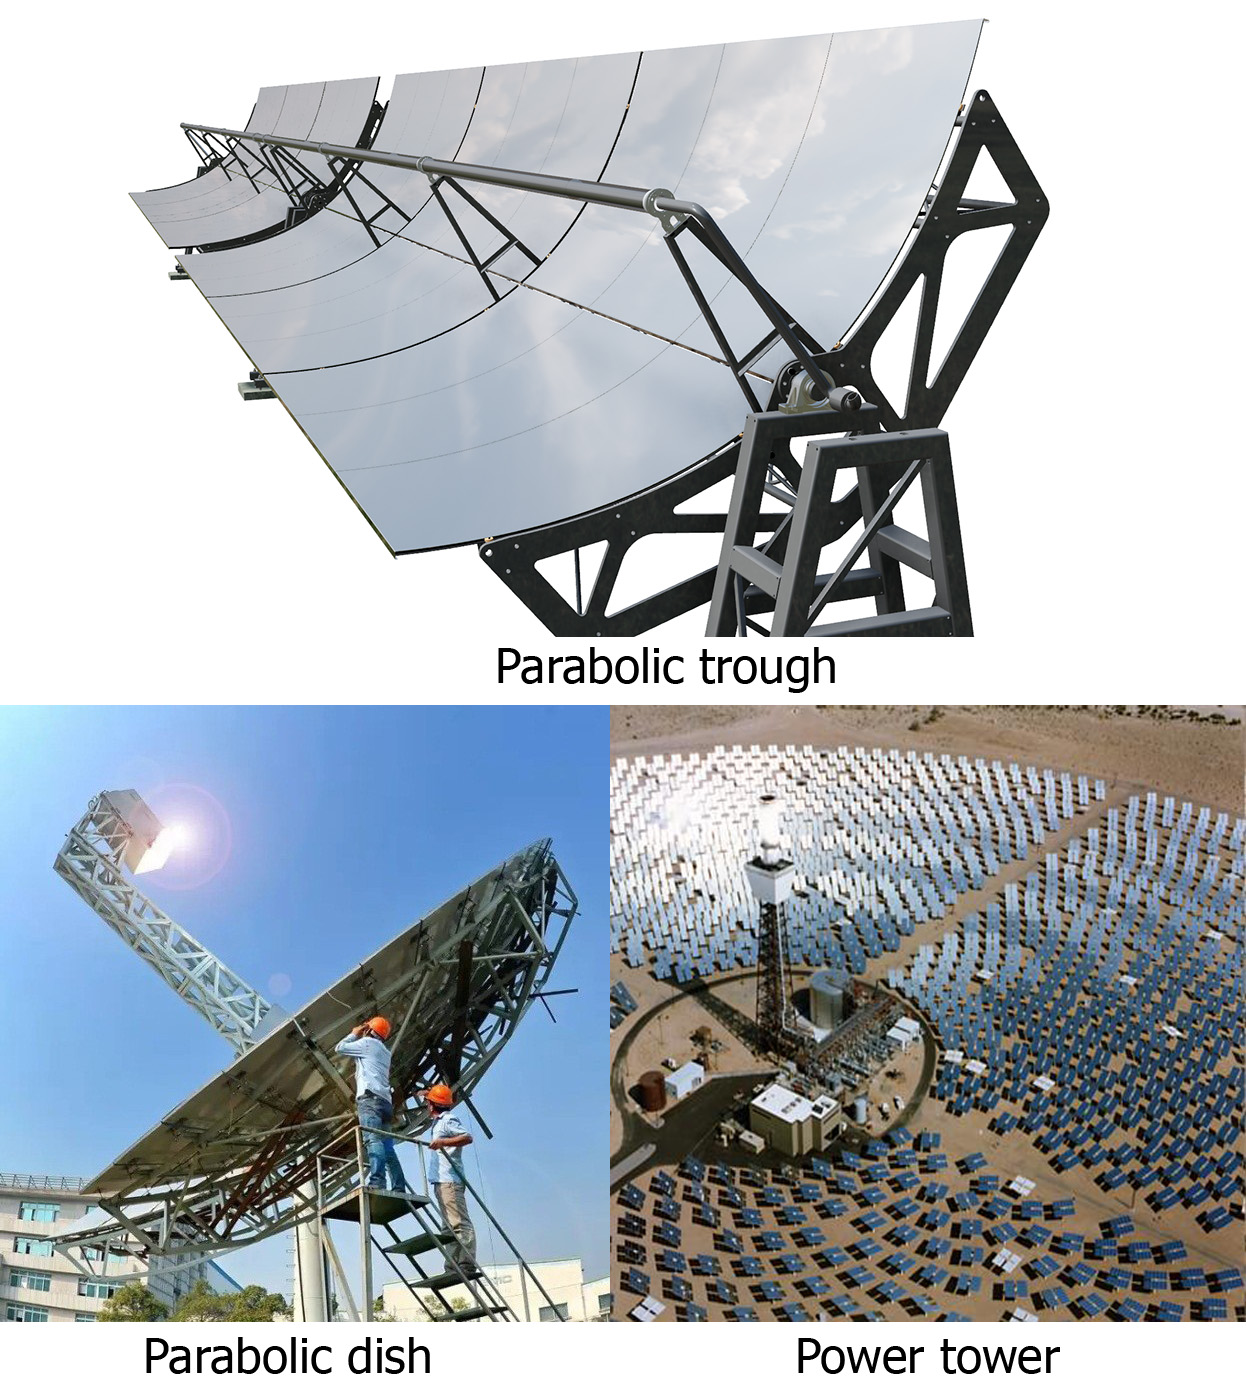
\includegraphics[width=.8\textwidth]{fig/Collectors}
\caption{三种CSP技术的应用实例}\label{fig:collectors}
\end{figure}

%A parabolic trough is a type of solar thermal collector whose mirror type is straight in one dimension and curved as a parabola in the other two. The reflector follows the sun during the daylight hours by tracking along a single axis. The energy of sunlight is reflected by the mirror and focused on the pipe positioned at the focal line. HTF (e.g. synthetic oil) runs through the pipe to absorb the heat generated by the focused sunlight, then used as the heat source for power generation or heating process.
太阳能槽式发电的反射镜是槽型抛物面。反射镜在白天采用单轴跟踪的形式跟踪太阳。反射镜将太阳光反射聚集到位于焦线处的集热管上。传热流体(例如合成油)流经集热管并吸收由聚集的太阳光产生的热量,然后为发电系统提供热量。

%A parabolic dish is a type of solar thermal collector whose mirror type is part of a circular paraboloid, which can converge the incoming sunlight traveling along the axis to the focus. Two-axis tracking system keeps it always directly towards the sun without cosine loss. It can obtain high concentration ratio and hence high temperature.
%Typically, a receiver or a Stirling engine is put at the focal point to absorb the converged energy. 
太阳能碟式发电的反射镜是旋转抛物面,它可以将沿着轴线照射的太阳光会聚到焦点上。碟式集热发电采用双轴跟踪系统来保证反射镜始终直接朝向太阳从而避免了余弦损失。它可以获得很高的聚光比,并因此获得高温热源。
通常情况下,焦点处放置有接收器或斯特林发动机来吸收会聚到的能量。

%Solar power tower is a type of solar furnace using a tower to receive the focused sunlight. It uses an array of flat, movable mirrors (called heliostats) to focus the sun's rays upon a collector tower. The heliostats track the sun on two axes (east to west and up and down). The receiver absorbs concentrated solar radiation and converts the solar energy into heat. The heat is then transferred to an HTF that carries the heat to a thermodynamic cycle for power generation. 
太阳能塔式发电是一种使用位于高塔顶部的接收器来接收聚焦阳光的太阳能发电形式。它使用大量可移动的太阳能反射镜(称为定日镜)。每台定日镜都各自配有跟踪机构将太阳光实时准确地反射到位于塔顶的接收器上。该跟踪机构为双轴跟踪(从东向西,向上和向下)跟踪太阳。接收器吸收集中的太阳辐射并将太阳能转换成热量,并将热量传递给传热流体,传热流体将热量传递至热力循环系统用于发电。
%Figure~\ref{fig:spt} shows the Solar Two power tower.
%\begin{figure}[!ht]
%\centering
%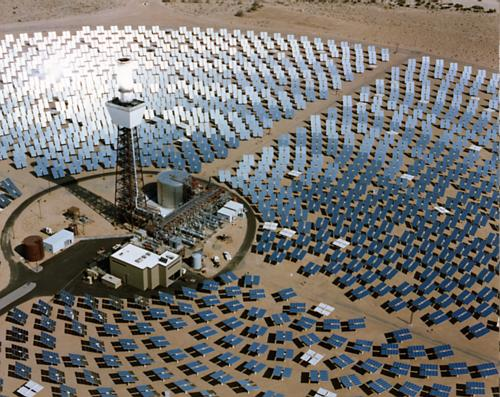
\includegraphics[width=.6\textwidth]{fig/PowerTower}
%\caption{Overall view of Solar Two power tower}\label{fig:spt}
%\end{figure}

%文献2
%In addition to wind and photovoltaic power, concentrating solar thermal power (CSP) will make a major contribution to electricity provision from renewable energies. Drawing on almost 30 years of operational experience in the multi-megawatt range, CSP is now a proven technology with a reliable cost and performance record. In conjunction with thermal energy storage, electricity can be provided according to demand. To date, solar thermal power plants with a total capacity of 1.3 GW are in operation worldwide, with an additional 2.3 GW under construction and 31.7 GW in advanced planning stage. Depending on the concentration factors, temperatures up to 1000°C can be reached to produce saturated or superheated steam for steam turbine cycles or compressed hot gas for gas turbine cycles. The heat rejected from these thermodynamic cycles can be used for sea water desalination, process heat and centralized provision of chilled water. While electricity generation from CSP plants is still more expensive than from wind turbines or photovoltaic panels, its independence from fluctuations and daily variation of wind speed and solar radiation provides it with a higher value. To become competitive with mid-load electricity from conventional power plants within the next 10–15 years, mass production of components, increased plant size and planning/operating experience will be accompanied by technological innovations. On 30 October 2009, a number of major industrial companies joined forces to establish the so-called DESERTEC Industry Initiative, which aims at providing by 2050 15 percent of European electricity from renewable energy sources in North Africa, while at the same time securing energy, water, income and employment for this region. Solar thermal power plants are in the heart of this concept.
% 现有发电技术的优缺点
% 梯级发电的意义

%Among the three solar thermal power technologies, parabolic trough is the most mature and commercially deployed technology. However, it has a low concentration ratio, the receiver's temperature is relatively low, the solar-to-electric efficiency is relatively low. Parabolic dish can obtain high temperature thermal energy, its solar-to-electric efficiency is higher than parabolic trough.
%Besides, one advantage of parabolic dish is that it requires much less water for power generation. However, solar parabolic dish is not a large-scale application, it's mainly applied for distributed power generation for its compact structure and easy installation. Solar power tower has a very high concentration ratio when more heliostats are used, the receiver's temperature can be very high and it can be applied for large-scale application. However, it has some disadvantages such as high investment and high system complexity. It is currently in rapid development stage.
在三种太阳能光热发电技术中,太阳能槽式发电是最成熟和最具商业化的技术。但是,它的聚光比较低,接收器的温度比较低,光热发电效率也比较低。太阳能碟式发电的聚光比达数百甚至数千,因此可以获得很高温度的热能,其光热发电效率高于太阳能槽式发电。此外,太阳能碟式发电的一个优点是它的发电过程用水量非常少。然而,太阳能碟式发电并未实现大规模应用,其结构紧凑,安装方便,主要应用于分布式发电。当使用大量的定日镜时,太阳能塔式发电的塔顶会聚了大量的能量,接收器的温度可以达到非常高,而且太阳能塔式发电也可以实现大规模应用。但与此同时,它也具有投资高,系统复杂度高的缺点。太阳能塔式发电目前处于快速发展阶段。

%It is very important to find out a way to utilize the advantages of existing solar thermal power technologies and overcome their disadvantages. In other words, to find out a new technology with higher efficiency and lower cost is urgent.
%This research is trying to achieve this by proposing a cascade system that uses different solar collectors and different thermodynamic cycles, which may be a new and feasible technology to realize large-scale, higher efficiency and lower cost solar thermal power generation.
不同种类的太阳能光热发电技术具有各自的优缺点,找到一种能够利用现有太阳能光热发电技术的优势并克服其缺点的方法是非常重要的。换句话说,开发出一种效率更高,成本更低的新的太阳能光热发电技术迫在眉睫。
本文试图通过提出使用不同型式的太阳能集热器和不同种类的热力循环的梯级系统来实现这一目标。这可能是实现大规模,高效率和低成本太阳能光热发电的新的可行技术。

%\section{State of the art}
\section{国内外研究现状}
% 范围的大小
%国内外对太阳能光热发电技术的研究现状。
%外文文献-问题-解决方案-本项目需求
%Solar thermal power technologies are getting more and more attention. 
%Many researchers have done lots of work to research and investigate it to increase its performance or reduce its cost.

%\subsection{Parabolic trough}
\subsection{太阳能槽式发电}

%Parabolic trough solar technology is the most proven and lowest cost large-scale solar power technology available.~\cite{Price2002}
抛物槽太阳能技术是目前最成熟和成本最低的大规模太阳能发电技术\cite{Price2002}。许多研究人员已经做了大量的工作来研究太阳能槽式发电,以提高性能或降低成本。其中很多研究着重于旨在测试抛物槽收集器的热性能和机械性能的实验性工作。

%Many of these works have concentrated on experimental work aimed at testing the mechanical and thermal performance of parabolic trough collectors. Dudley et al.~\cite{Dudley1994} tested the collector efficiency and thermal losses of the LS-2 type trough collector. Burkholder and Kutscher~\cite{Burkholder2009} tested the heat losses of Solel's UVAC3 and Schott's 2008 PTR70 parabolic trough collectors. A correlation to estimate the thermal efficiency of the collectors as a function of the absorber temperature was developed. Reddy et al.~\cite{Reddy2015b} developed and investigated six different receiver configurations of trough collectors for performance comparison. Experimental tests were carried out for a 15$\,\mathrm{m^2}$ collector according to ASHRAE 93-1986 test procedure.
%Li et al.~\cite{Li2015} carried out experiments to verify the feasibility of proposed end loss compensation methods. A fan-shaped plane mirror was put at one end of the trough collectors to compensate the end loss effect. Results prove that the compensation methods are feasible and effective.
来自桑迪亚国家实验室的Dudley等人\cite{Dudley1994}测试了应用于SEGS太阳能光热电站的LS-2型槽式接收器的集热效率和热损失。实验分析了不同类型的选择性涂层,不同接收器配置,不同真空度对集热器性能的影响。他们还建立了槽式接收器的一维分析模型,并将模拟结果与实验数据进行了对比分析。

来自美国国家可再生能源实验室的Burkholder和Kutscher\cite{Burkholder2009}测试了来自Solel的UVAC3型槽式集热器和来自Schott的PTR70型槽式集热器,并建立了以接收器平均温度和环境温度为参数的热损失方程。

Kr\"uger等~\cite{Kruger2008}对Solitem PTC 1800型槽式集热器的光学性能进行了研究,并以工作温度为200$^\circ\mathrm{C}$的高压水作为传热流体进行了实验分析,并对光学效率的改进提出了建议。

Reddy等\cite{Reddy2015b}开发并研究了六种不同型式的槽式接收器,并进行了性能对比分析。根据ASHRAE 93-1986测试程序,针对一台集热面积为15$\,\mathrm{m^2}$的集热器,对六种不同型式的接收器进行了实验测试分析。实验表明,多孔圆盘型接收器可以显著提高槽式集热器的性能,可以有效地用于工业加热过程。

%众所周知,实验研究最具有说服力和可信性,然而,实验研究需要大量的研发成本和实验时间,所以槽式太阳能光热发电的大部分工作都采用模拟分析的方法,通过建造相关模型,对槽式集热器进行研究,或是通过实验对所建立的模型及方法进行相关的验证工作。
%It is well known that experimental studies are the most accurate and convincing method for parabolic trough collector research. However, this method is not only investment required and also time consuming. In order to reduce the R\&D cost and time, parabolic trough collectors are usually modeled.

% 光学效率
一些研究人员研究了槽式集热器的光学效率模型。王金平等\cite{Wang2016}提出了用于计算槽式集热器的光学效率的数学模型,并选取了中国的三个典型地区作为实验地点,进行了相关的实验验证工作。结果表明,其提出的光学效率数学模型的相对误差在1\%到5\%之间。
邹斌等\cite{Zou2017}研究了太阳形状和入射角对槽式集热器的性能影响,发现太阳形状对光学效率具有很大的影响,需要在实际应用中考虑此因素。更宽的开口和更细的吸收管将使入射角对端部损失的影响更大。他们还发现,对于特定集热器存在着最佳焦距使光学效率获得最大值。
L\"upfert等\cite{Lupfert2006}介绍了实际工程应用中用于分析槽式集热器的形状参数和光学参数的技术,并对槽式集热器的集热器形状测量、光通量测量、光线跟踪、热性能分析等的数据进行了分析。结果表明,不同的测量方法和参数分析可以获得一致的结果,这些结果可以为下一代测量技术和分析方法提供相关参考。
许成木等\cite{Xu2014}分析了南北布置的槽式集热器的光学效率,并提出了一种补偿端部损失的方法,并推导出了端部损失比例与采用补偿损失方法后效率增加量之间的计算公式。计算分析了不同纬度的日光学损失率,年光学损失率,以及采用补偿损失方法后的日增光学效率和年增光学效率。结果表明,该补偿方法对于维度高于25度的地区的短集热器非常适用。
黄卫东等\cite{Huang2012}提出了一种新的光学性能分析模型,该模型采用了改进的积分算法,用于模拟带有真空管的槽式接收器的性能。首先推导了反射镜各点光学效率的解析方程,然后用数值积分算法模拟了系统的光学效率。可以通过该程序计算出余弦损失,集热效率,热损失。

%热效率和㶲效率分析,想要从能量利用的数量和品质上提升槽式集热器的性能。
一些学者对槽式系统进行了热效率和㶲效率分析,以便于从能量利用的数量和品质上提升槽式系统的性能。
Padilla等\cite{Padilla2014}在其建立的传热模型\cite{Padilla2011}的基础上进行了㶲效率分析,来研究实验操作和环境参数对槽式集热器性能的影响。分析考虑了传热流体的入口温度,质量流量,风速,真空压力以及太阳直射辐射强度等因素,结果表明,传热流体的入口温度,太阳直射辐射强度和真空度对散热性能有显着影响,但传热流体的流量和风速的影响很小。如果传热流体入口温度固定,则不能同时获得最大的热效率和㶲效率,它们呈现相反的变化趋势。最后,他们发现最大㶲损发生在接收器与太阳之间的辐射传热过程中。
郭江峰等\cite{JiangfengGuo2016-1}研究了一些参数对槽式集热器的热效率和㶲效率的影响。结果发现,当传热流体的质量流量,环境温度和入射角增大时,太阳鞥接收器的热损失减少。随着传热流体入口温度,风速和玻璃管内径的增加,槽式接收器的㶲损失也随之增加。当入射角较大时,存在最佳的传热流体流量使㶲效率获得最大值。

%热效率模型
一些研究人员致力于使用新方法开发出精度更高的槽式系统模型。Behar等\cite{Behar2015}开发并验证了一种新颖的槽式集热器模型。通过与桑迪亚国家实验室和国家可再生能源实验室建立的模型进行的比较,该模型显示出更好的集热效率预测精度。
Padilla等\cite{Padilla2011}针对槽式集热器建立了详细的一位数值模型分析。为了求解换热过程中的数学模型,偏微分方程被离散化,然后通过求解非线性代数方程得到槽式集热器的数值分析结果。该模型得到的数值结果利用桑迪亚国家实验室的试验数据进行了验证。
Hachicha等\cite{Hachicha2013}基于有限体积法建立了一个详细的一维槽式集热器模型。该模型还采用了光线追踪法,并考虑了太阳大小带来的影响。该模型通过文献上的数据进行了验证,和其它模型及实验结果具有很好的一致性。
郭江峰与淮秀兰~\cite{JiangfengGuo2016-2}基于基因算法对槽式接收器进行了多目标参数优化研究,该研究同时以热效率和㶲效率为优化目标。
Boukelia等\cite{Boukelia2016}研究了三种应用于的人工神经网络的不同形式的前馈向后传播学习算法,包括Levenberge Marguardt法、扩展共轭梯度法和Pola-Ribiere共轭梯度法,并利用这些算法对槽式电厂进行预测和技术经济优化。
刘启斌等\cite{Liu2012}开发了基于最小二乘支持向量机(LSSVM)方法的槽式集热器模型并通过数值模拟评估了LSSVM方法的可行性和有效性。
Lobon等\cite{Lobon2014}引入了计算流体动力学特性的模拟方法来预测槽式系统中蒸汽发生系统,该蒸汽发生系统位于西班牙Plataforma Solar de Almeria。利用CFD代码包STAR-CCM+建立了一个有效的多相流体模型,可以模拟槽式集热器中的多相流体的动力学行为。模拟结果和试验数据在各种工作条件下进行了对比分析。
为了得到槽式集热器的动力学特性,并计算出散热损失,Mohamad等\cite{Mohamad2014}分析了工作流体,吸热管和玻璃管沿轴向的温度分布。结果发现,使用双层玻璃罩可以有效提高高温运行时的集热效率。然而,当集热器的长度小于10$\,\mathrm{m}$时,使用单层玻璃罩比双层玻璃罩更经济。结果还清晰地表明,随着吸热管管径的增大,热损失也迅速增加。
郭苏等\cite{SuGuo2016}针对槽式系统中的直接蒸汽生产系统开发了一个非线性分布的参数模型来模拟在全部或部分太阳辐射干扰下的直接蒸汽生产系统的动态特性。该模型具有两个优点:(1)传热系数和摩擦阻力系数采用实时局部值;(2)考虑收集器的完整回路,包括过冷区,蒸发区和过热区。该模型已经使用新南威尔士大学太阳能热能实验室的实验数据进行验证,出口流体温度相对误差仅为1.91%。

% 其它用法
一些研究人员还提出了新的太阳能槽式系统。Ashouri等\cite{Ashouri2015}将一台小型抛物槽式集热器,一台储热罐和一台辅助加热器连接到一个卡林纳循环,并研究了其全年热力性能和全年经济性能。
% 空气介质

Good等提出了使用空气作为槽式集热器的集热方案,空气的集热温度可以达到600$\mathrm{^\circ C}$。吸热管有一组螺旋卷曲的金属管组成,外层包裹着矩形截面的绝缘槽。该方案采用二次反射镜面将聚光比提升至97。
Bader等\cite{Bader2015}针对采用空气作为传热介质的槽式真空接收器建立了数值模型。该模型考虑了四种不同的接收器型式,包括光滑圆管吸热管和V型吸热管,单层套管和双层套管。数值模型考虑了不同类型的热损失以及吸热管内的温度分布。
% 强化换热
Kaloudis等\cite{Kaloudis2016}利用CFD软件对采用含有纳米颗粒的流体作为传热介质的槽式集热器进行了模拟分析。使用Syltherm 800作为流体,在其中加入了浓度为0\%到4\%的氧化铝纳米颗粒。结果发现,当纳米颗粒浓度为4\%时,系统的集热效率可以达到10\%的提升。

% 新颖的系统
%Tan et al.~\cite{Tan2014} proposed a two-stage photovoltaic thermal system based on solar trough concentration, in which the metal cavity heating stage is added on the basis of the PV/T stage, and thermal energy with higher temperature is output while electric energy is output. The experimental platform of the two-stage photovoltaic thermal system was established, with a 1.8 m$^2$ mirror PV/T stage and a 15 m$^2$ mirror heating stage, or a 1.8 m$^2$ mirror PV/T stage and a 30 m$^2$ mirror heating stage. The results show that with single cycle, the long metal cavity heating stage would bring lower thermal efficiency, but temperature rise of the working medium is higher, up to 12.06$\mathrm{^\circ C}$ with only single cycle. With 30 min closed multiple cycles, the temperature of the working medium in the water tank was 62.8$\mathrm{^\circ C}$, with an increase of 28.7$\mathrm{^\circ C}$, and thermal energy with higher temperature could be output.
Al-Sulaiman等\cite{AlSulaiman2012}基于槽式集热器和有机工质朗肯循环提出了一种冷热电三联供的新型系统,并对系统的效率、电功率、供热供冷比进行了性能评估。研究表明,太阳能模式的最大发电效率是15\%,太阳能和蓄能联供模式的最大发电效率是7\%,只是用蓄能模式是6.5\%。太阳能模式的冷热电三联供最高效率为94\%,太阳能和蓄能联供模式为47\%,只使用蓄能模式为42\%。
\nomenclature[C]{CCHP}{Combined cooling, heating and power}
\nomenclature[C]{HTF}{Heat Transfer Fluid}
\nomenclature[C]{CFD}{Computational fluid dynamics}
\nomenclature[C]{DSG}{Direct Steam Generation}
\nomenclature[C]{LM}{Levenberge Marguardt}
\nomenclature[C]{SCG}{Scaled Conjugate Gradient}
\nomenclature[C]{PCG}{Pola-Ribiere Conjugate Gradient}
\nomenclature[C]{ANN}{Artificial neural network}
%\nomenclature[C]{PTSTPP}{Parabolic Trough Solar Thermal Power Plant}
\nomenclature[C]{SRC}{Steam Rankine Cycle}
\nomenclature[C]{ORC}{Organic Rankine Cycle}
\nomenclature[C]{PTC}{Parabolic Trough Collector}
\nomenclature[C]{SNL}{Sandia National Laboratory}
\nomenclature[C]{LSSVM}{Least squares support vector machine}

\subsection{Parabolic dish}
\label{sec:pd}

The solar parabolic dish system is known for its highest efficiency of all solar technologies (around 30\%). It is suitable for distributed power generation for its compact structure and easy installation.  

Many researchers conducted experiments to investigate the solar parabolic dish system or to validate proposed models.
To investigate the heat loss of semi-spherical cavity receiver applied for solar parabolic dish system, Tan et al.~\cite{Tan2014b} conducted experiments with different fluid inlet temperatures, receiver inclination angles and aperture sizes. Correlations of Nusselt number as a function of Grashof number were developed by the experiment results.
Chaudhary et al.~\cite{Chaudhary2013} investigated a solar cooker based on dish collector with phase change thermal (PCM) storage unit. Three cases have been considered for the investigation: ordinary solar cooker, solar cooker with outer surface painted black, and solar cooker with outer surface painted black along with glazing. It was observed that the last case shows the best performance, which can store 32.3\% and 26.8\% more heat for the PCM compared with the first and second cases respectively.
Mawire and Taole~\cite{Mawire2014} investigated the thermal performance of a cylindrical cavity receiver for an SK-14 parabolic dish concentrator. The receiver exergy rates and efficiencies are found to be appreciably smaller than the receiver energy rates and efficiencies. The exergy factor is found to be high under conditions of high solar radiation and high operating temperatures. An optical efficiency of around 52\% for parabolic dish system is determined under high solar radiation conditions.
Zhu et al.~\cite{Zhu2015} conducted an experimental investigation of a coil type solar dish receiver. The solar irradiance is about 650$\,\mathrm{W/m^2}$, while the concentrated solar flux at the aperture is approximately 1000$\,\mathrm{kW/m^2}$. The energy and exergy performance of the receiver was analyzed and the experimental results show that, at steady state, the energy efficiency is maintained around 80\%, and the exergy efficiency is around 28\%. 
CRTEn developed a solar dish system using four types of absorbers: flat plat, disk, water calorimeter and solar heat exchanger.~\cite{Skouri2013} For the different types of absorbers, experiments were conducted to obtain the mean concentration ratio and both energy and exergy efficiency. Results shown that thermal energy efficiency of the system varies from 40\% to 77\%, the concentrating system reaches an average exergy efficiency of 50\% and a concentration factor around 178.
Thirunavukkarasu et al.~\cite{Thirunavukkarasu2017} carried out an experimental study to investigate the thermal performance of a cavity receiver for a dish concentrator. The overall system efficiency of the solar collector is 69.47\%. The average exergy efficiency of the receiver is found to be 5.88\% with a peak value of 10.35\%.
Pavlovic et al.~\cite{Pavlovic2017} performed the experimental study of a solar dish system. In this system, different working fluids (water, thermal oil and air) were used to validate the numerical models developed in EES (Engineering Equation Solver). It was found that water is the most appropriate working fluid for low-temperature applications, while thermal oil is the most appropriate working fluid for higher-temperature applications.

Some researchers focused on the dish concentrator, many proposed different shapes of concentrators. The perfect concentrator has a parabolic shape, but for some considerations (better production, safer transportation, lest cost and so on), some solar concentrators are composed of multiple spherically shaped mirrors.
A large dish solar concentrator, SG3, which is about 400$\,\mathrm{m^2}$, was designed and demonstrated in Australian National University in 1994 as shown in Figure~\ref{fig:LargeDish}.~\cite{Lovegrove2011} It successfully proved the technical viability of a concentrator that is approximately three times bigger than any other produced. 
\begin{figure}[!ht]
\centering
\includegraphics[width=.8\textwidth]{fig/largeDish.jpg}
\caption{The SG3 400$\,\mathrm{m^2}$ dish in Australian National University}\label{fig:LargeDish}
\end{figure}
Berumen et al.~\cite{Berumen2004} developed a refector consists of 12 facets made of fiberglass with a reflecting surface made of aluminum sheet with reflectance of 86\%.
Pavlovic et al.~\cite{Pavlovic2014} presented a procedure to design a square facet concentrator for laboratory-scale research on medium-temperature thermal processes. A parabolic collector made up of individual square mirror panels (facets) were investigated. These facets can deliver up to 13.604 kW radiative power over a 250$\,\mathrm{mm}$ radius dish receiver with average concentrating ratio exceeding 1200.
Hijazi et al.~\cite{Hijazi2016} designed a low cost parabolic solar dish concentrator with small-to moderate size for direct electricity generation and special attention is given to the selection of the appropriate dimensions of the reflecting surfaces.
Ma et al.~\cite{Ma2012} designed a solar dish concentrator based on triangular membrane facets. A 600-facet concentrator with focal-diameter ratio of 1.1 will achieve 83.63\% of radiative collection efficiency over a 15$\,\mathrm{cm}$ radius disk located in the focal plane, with a mean solar concentration ratio exceeding 300.
A 3.6-meter diameter stretched-membrane optical facet for a parabolic dish has been successfully designed and demonstrated under contract with Sandia National Laboratories.~\cite{Schertz1991} Twelve facets identical to them will be used to make the lightweight reflector of the dish. The project goal of 2.5$\,\mathrm{mrad}$ surface accuracy was met with each of the two full-sized prototypes, and accuracies of as low as 1.1$\,\mathrm{mrad}$ were achieved.

Many researches investigated the flux distribution and thermal performance of the solar dish receiver.
Shuai et al.~\cite{Shuai2010} developed a flux distribution measurement system for dish concentrators. A charge coupled device camera was applied to obtain the contours of the flux distribution for target placements with different location. Further, the measured flux distributions are compared with a Monte Carlo-predicted distribution. The results can be a valuable reference for the design and assemblage of the solar collector system.
Mao et al.~\cite{Mao2014b} simulated the flux distribution of a dish receiver using MCRT method. The impacts of incident solar irradiation, aspect ratio (the ratio of the receiver height to the receiver diameter), and system error on the radiation flux of the receiver are investigated.
Li et al.~\cite{Li2011b} used the Monte-Carlo ray-tracing method for the radiation flux distribution of the solar dish receiver system. The result was validated by experiment and used as the boundary conditions of a CFD receiver model. The fluid flow and conjugate heat transfer in the receiver was numerically simulated and validated by experiments.
Wang and Laumert~\cite{Wang2017} used the ray-tracing methodology to investigate the effects of cavity surface materials on the flux distribution for an impinging receiver. Five cavity surface materials and their combinations have been studied. The results show that the flux distribution and the total optical efficiency are much more sensitive to the absorptivity on the cylindrical surface than on the bottom.
Blazquez et al.~\cite{Blazquez2016} studied the optimization of the concentrator and receiver cavity geometry of parabolic dish system. Ray-tracing analysis has been performed with the open source software Tonatiuh, a ray-tracing tool specifically oriented to the modeling of solar concentrators.
Reddy et al.~\cite{Reddy2015,Reddy2015b} performed the theoretical thermal performance analysis of a fuzzy focal solar parabolic dish concentrator with modified cavity receiver. Total heat loss from the modified cavity receiver was estimated considering the effects of wind conditions, operating temperature, emissivity of cavity cover and thickness of insulation. Time constant test was carried out to determine the influence of sudden change in solar radiation at steady state conditions. The daily performance tests were conducted for different flow rates.
Vikram and Reddy~\cite{Vikram2015} used a three-dimensional numerical model to investigate the total heat losses of three modified cavity with three configurations for parabolic dish receiver. The effects of cavity diameter ratio, tilt angle, operating temperature, insulation thickness and emissivity on the heat loss of the modified cavity receiver were studied. Based on artificial neural network (ANN) modeling, an improved Nusselt number correlation was proposed for convection, radiation and total heat loss calculation.

Some researchers focused on the solar tracking system.
Patil et al.~\cite{Patil2016} described the development of automatic dual axis solar tracking system for solar parabolic dish. Five light dependent resistors were used to sense the sunlight and two permanent magnet DC motors are used to move the solar dish. A controller software were developed to control the motors using the data sensed by the resistors.
Raturi et al.~\cite{Raturi2014} proposed a solar tracking system based on gravity which does not require any external source of power. The prototype test results and analysis show that the system can run successfully.
Kuang and Zhang~\cite{Kuang2012} developed new design and implementation of tracking system to improve tracking accuracy for dish solar based on embedded system that mixes active and passive tracking.
Jin et al.~\cite{Jin2013} described a two-axis sun tracking system with PLC (programmable logic controller) controlled and a combinative tracking method combined active and passive tracking methods for higher accuracy.
Shanmugam and Christraj~\cite{Shanmugam2005} presented a method of intermittent tracking of the sun in the north-south direction with no tracking in the east-west direction for less energy yield and the frequency of tracking in the north-south direction determined by variations in solar altitude angle and size of the absorber in paraboloidal dish concentrator.
\nomenclature[C]{MCRT}{Monte Carlo Ray Tracing}
\nomenclature[C]{CRTEn}{Research and technologies centre of energy in Borj Cedria}

\subsection{Power tower}
\label{sec:st}

Solar power tower technology is gaining more and more interest for its large scale, high concentration ratio and high operating temperature.
It is widely regarded as the most promising solar thermal power technology.

Advances in the power tower technology are mainly the component update as well as system improvement.
Some researchers focused on the choice of HTF that used in the power tower. 
One already standardized commercial plant cycle is the solar tower with conventional steam cycle.~\cite{Spiros2017} Steam is 
used as both HTF and working fluid in the Rankine cycle. Steam is directly generated in the receiver and flows into the steam turbine for power generation.~\cite{Montes2009,Feldhoff2012,Steinmann2006,Yu2017,Gonzalez2017} Many researchers concerned about using other fluids (molten salt, air) as HTF.
Toto et al.~\cite{Toro2016} proposed an idea of a hybrid power tower using air as the working fluid of a topping Brayton cycle and HTF of a bottoming Rankine cycle.
Rold~\cite{Rold2016} proposed an idea of using supercritical CO$_2$ as HTF. A simplified CFD model has been built to analyze the feasibility of supercritical CO$_2$ as HTF in solar towers. It was found that it is a promising alternative for both better operating conditions and lower maintenance cost.
Joshi et al.~\cite{Joshi2016} used the dynamic simulation technology to evaluate a molten salt central receiver design and control strategies.

Many researchers concerned about the heliostats to reach high tracking accuracies under wind loads and thermal stress situations. On the other hand, trade-off between higher land utilization and lower block ratio is also a hot spot.
% 定日镜
Thalange et al.~\cite{Thalange2017} presented the protocol and results of systematic structural analysis of tripod heliostats to reduce the cost and enhance the mechanical behavior.
Besarati and Yogi~\cite{Besarati2014} developed a new and simple method to improve the calculation speed and accuracy for shading and blocking computation of the heliostat field. The Sassi method~\cite{Sassi1983} is used for the shading and blocking efficiency. A 50$\,\mathrm{MWth}$ heliostat field in Dagget, California, USA was used as a case study for the proposed method.
Wei et al.~\cite{Wei2010} proposed a new method for the design of the heliostat field layout for solar tower power plant. Based on the new method, a new code for heliostat field layout design (HFLD) has been developed and a new heliostat field layout for the PS10 plant at the PS10 location has been designed using the new code. Compared with current PS10 layout, the new designed heliostats has the same optical efficiency but with a faster response speed.

Some researchers concerned about the performance of central receiver of power tower.
Kim et al.~\cite{Kim2015} investigated the heat loss of solar central receiver. Numerical simulations using CFD (Computational Fluid Dynamics) with the consideration of four different receiver shapes were carried out to get the influence on convection and radiation heat losses. Different opening ratio between cavity aperture area and receiver aperture area, receiver temperatures, wind velocities and wind directions (head-on and side-on) were considered for the simulations. Results were used to get a simplified correlation model which gets the fraction of convection heat loss. The correlation obtained shows good agreements with the simulation results. The correlation was also validated with experimental data from three central receiver systems (Martin Marietta, Solar One and Solar Two).
Lara et al.~\cite{Lara2016} presented a novel modeling tool for calculation of central receiver concentrated flux distributions. The modeling tool is based on a drift model that includes different geometrical error sources in a rigorous manner and on a simple analytic approximation for the individual flux distribution of a heliostat. 

%Haroun~\cite{El2015} proposed a novel system combines both solar chimney and solar tower. The solar tower receiver was installed at the top of the chimney. Theoretical study of this novel system was conducted. The results shown that the new system generates more power than conventional system with the same parameters of solar irradiance, collector radius, height of chimney, and height of solar tower. The inlet air speed of the chimney is higher than that of the conventional, and it increases with the solar irradiance. Moreover, the results indicated that there exists a optimum ratio of solar tower height to solar chimney height for the maximum overall power.
Some researchers devoted on the simulation of power tower plants.
Franchini et al.~\cite{Franchini2013} developed a computing procedure for solar tower system under both nominal and part load conditions. A Siemens gas turbine product, SGT-800, was applied for the Integrated Solar Combined Cycle (ISCC) as a study case for the solar tower system. The turbine has a dual pressure heat recovery steam generator, which can be used for the Integrated Solar Combined ISCC plant. A model of Solar Rankine Cycle (SRC) driven by power tower was also developed for comparison. A highest solar-to-electric efficiency of 21.8\% can be achieved by the designed ISCC plant. And in all conditions, the global solar energy conversion efficiency of the ISCC is higher than that of the SRC.
Xu et al.~\cite{Xu2011a,Xu2012} created a model of the 1 MW Dahan solar thermal power tower plant using the modular modeling method. The dynamic and static characteristics of the power plant are analyzed based on these models. Response curves of the system state parameters are given for different solar irradiance disturbances. Conclusions in this paper are good references for the design of solar thermal power tower plant.
Benammar et al.~\cite{Benammar2014} developed a mathematical model based on energy analysis for solar tower power plants. A general nonlinear mathematical model of the studied system  has been presented and solved using numerical optimization methods. The analysis of these results shows the existence of an optimal receiver efficiency value for each steam mass flow, receiver surface temperature and receiver surface area.
\nomenclature[C]{ISCC}{Integrated Solar Combined Cycle}

\subsection{梯级太阳能光热发电}
\label{sec:cs}

为了更加有效地利用太阳能光热发电系统中各部件的特性,许多研究人员研究了梯级太阳能系统。梯级太阳能系统的研究主要有两个方向:一个是梯级收集,一个是梯级利用。
%To fully utilize the features of components of solar thermal power system, cascade solar systems are researched by many researchers. There are mainly two directions of the research of cascade solar systems. One is cascade collection, the other is cascade utilization.

\subsubsection{梯级收集}

许多研究人员研究了在太阳能光热发电技术中采用多种集热器实现太阳能梯级收集的方案。Suzuki\cite{Suzuki1986}分析了使用两种不同型式的集热器串联连接的集热方案。研究表明,集热器的一个参数值——集热效率和光学效率的乘积,是决定梯级系统是否比单独使用任何一种集热器更高效的关键参数。如果更低聚光比的集热器的这个参数值比更高聚光比的这个参数值大,那么梯级系统更加高效。此外还发现,梯级系统具有最佳的运行参数。

Kribus等\cite{Kribus1999}提出了多级独立开口的方案来利用太阳辐射的不均匀分布。传热流体一次经过辐射能量密度递增的接收器来实现逐级加热。为了验证这种方案,他们在魏茨曼研究所的太阳能塔的塔顶放置了一个双级接收器。在该接收器中,空气作为传热流体在低温级中被加热至750$\mathrm{^\circ C}$,然后流入高温级被加热至1000$\mathrm{^\circ C}$。该双级接收器的结构图如图\ref{fig:Kribus1999}所示。

\begin{figure}[!ht]
\centering
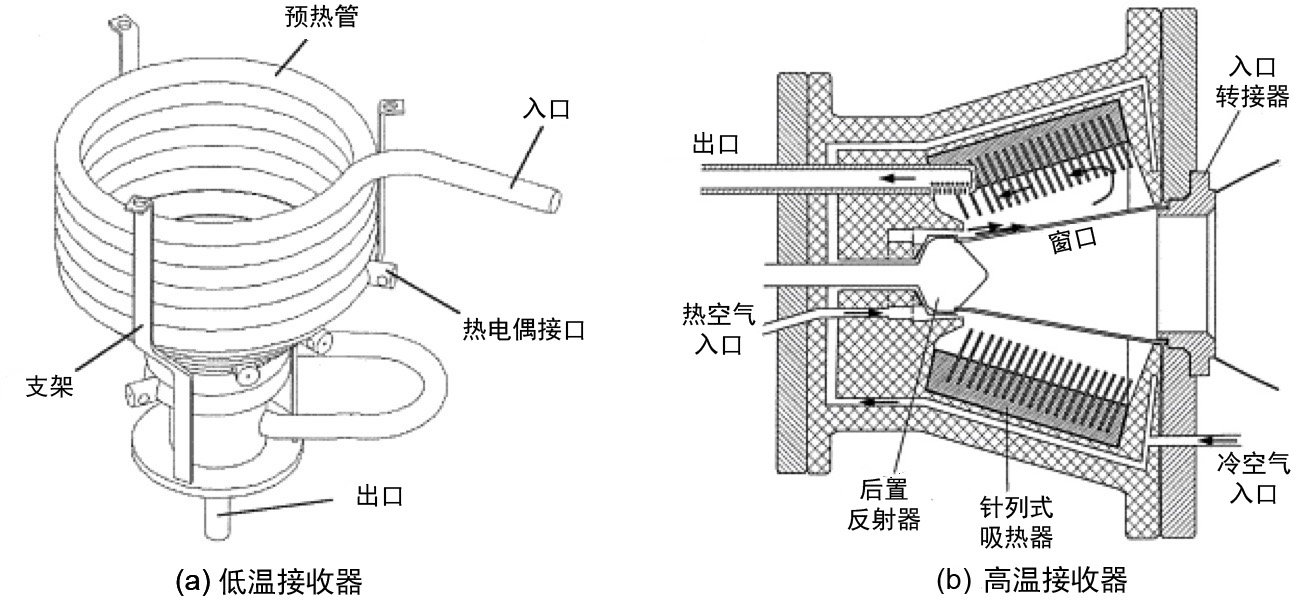
\includegraphics[width=.8\textwidth]{fig/Kribus1999.jpg}
\caption{双级集热器的结构图}
\label{fig:Kribus1999}
\end{figure}

% 组合使用不同厂家的集热器
Gordon和Saltiel提出了一种分析方法来预测采用多种型式集热器(“多级系统”)的光热系统的长期性能。该分析方法允许设计者针对给定负荷,来决定使用组合不同型式集热器的最有效的方法。一个成功的实例证明了该方法可以有效节省“多级”系统的成本。

Oshida和Suzuki\cite{Oshida1987}提出了利用不同类型集热器实现梯级集热的思想。梯级系统中使用两个吸热器,分为低温吸热器和高温吸热器,其中低温吸热管由费列尔镜片加热,高温吸热管由槽式镜面加热。传热流体先流经低温吸热器完成预热,再在高温吸热器中完成进一步加热。传热流体可以在该梯级系统中更加高效地完成加热过程。

Desai等\cite{Desai2015}提出了一种集成太阳能集热方案,该方案同时采用槽式集热器和线性费列尔集热器。采用集成集热热方案的系统结构图如图\ref{fig:Desai2015}所示。对采用集成集热方案的电厂进行了热力学和经济学分析,并同基于槽式集热器的电厂和基于线性费列尔集热器的电厂进行了对比。结果表明,采用集成方案的电厂的发电成本要比基于槽式集热器的电厂低9.6\%,比基于线性费列尔集热器的电厂低13.5\%。

\begin{figure}[!ht]
\centering
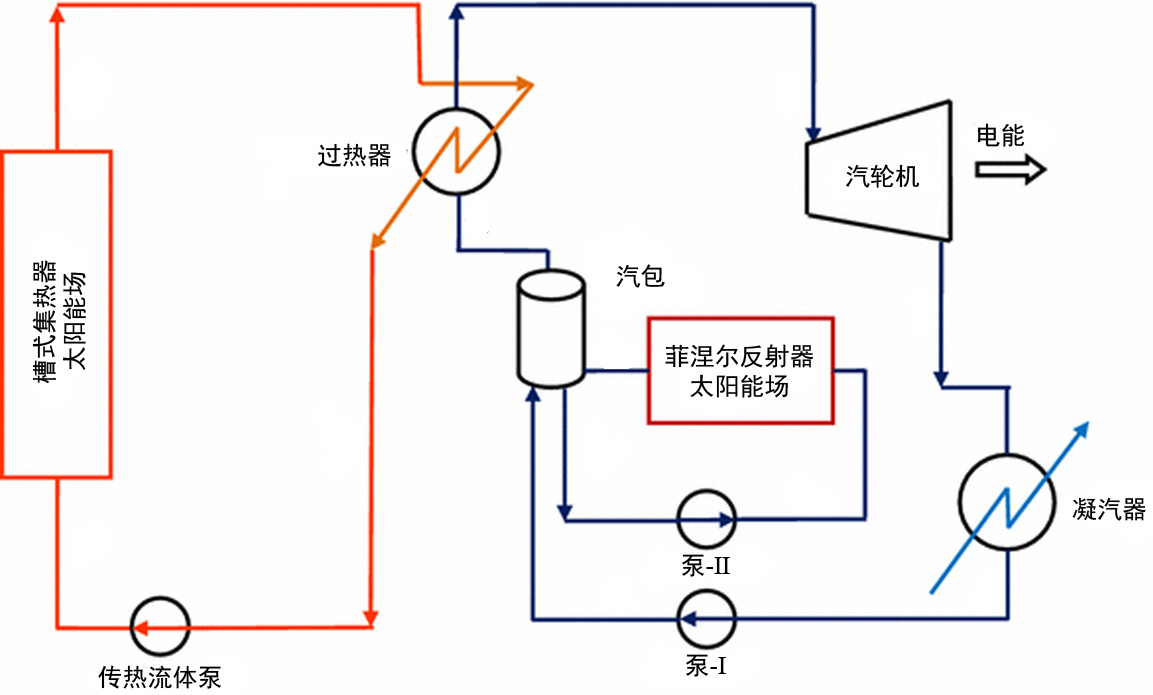
\includegraphics[width=.7\textwidth]{fig/Desai2015.jpg}
\caption{采用集成集热热方案的系统结构图}\label{fig:Desai2015}
\end{figure}

Coco等\cite{Coco2015}为集成了直接蒸汽生产系统和布雷顿循环的系统提出了四种不同的线性集热太阳能光热发电方案。在这些方案中,太阳能场被分成了不同的片区来满足不同的集热需求。这种思想为在太阳能场中使用多种型式的集热器提供了可行性。

\nomenclature[C]{CPC}{Compound parabolic collector}

\subsubsection{梯级利用}
%利用槽式集热器为塔式电站的给水预热
%朗肯循环、斯特林循环综合利用
%多级朗肯循环

Many researchers have done the work on the combination of different thermodynamic cycles for CSP. 
Lots of the work focused on integrated solar combined cycle (ISCC) with parabolic trough, where Rankine cycle is used as the bottom cycle.
很多学者致力于在太阳能光热发电系统中组合使用多种热力循环来实现能量的梯级利用。其中大部分的工作聚焦于综合太阳能联合循环(ISCC),在该循环中,朗肯循环作为底部循环,布雷顿循环作为顶部循环。

李元媛和杨勇平\cite{Li2014}提出了一种新颖的ISCC系统,可以实现高达30\%的光电转换效率,其系统结构图如图\ref{fig:Li2014}所示。他们分析了将收集到的太阳能用于ISCC系统不同位置对系统整体性能的影响,结果表明,将太阳能用于蒸发过程可以获得最大的系统整体性能。
\begin{figure}[!ht]
\centering
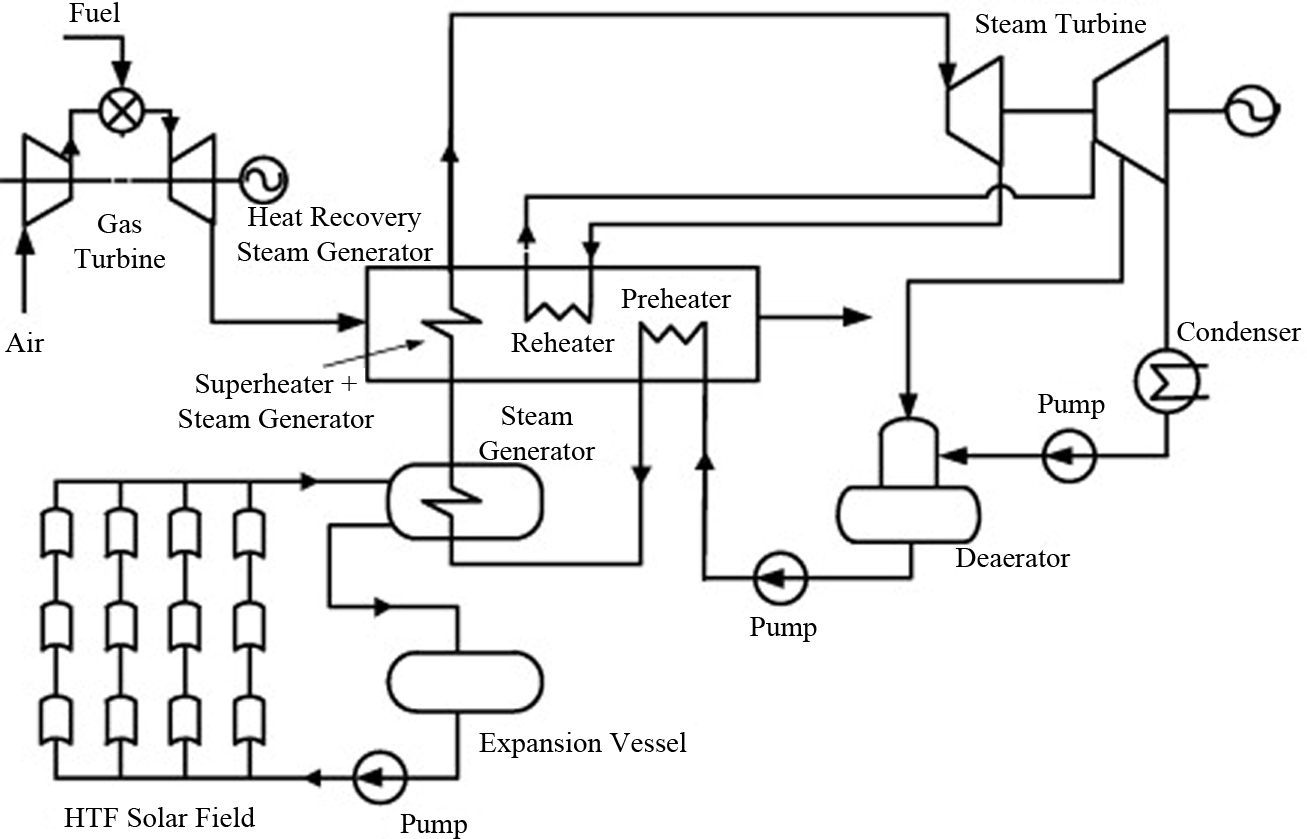
\includegraphics[width=.8\textwidth]{fig/Li2014.jpg}
\caption{李元媛和杨勇平提出的ISCC系统结构图}
\label{fig:Li2014}
\end{figure}

G\"{u}len使用了热力学第二定律中的㶲概念来简化ISCC系统的优化过程。经过㶲分析,为ISCC设计提供了基于物理方程的,对用户友好的指导方针。

Shaaban\cite{Shaaban2016}介绍了一种新型的ISCC系统,该系统同时考虑使用水工质朗肯循环和有机工质朗肯循环作为底部循环,其系统结构图如图\ref{fig:Shaaban2016}所示。有机工质循环用于冷却压缩空气,并利用这部分热量产生一部分电能。还研究了采用不同有机工质对该新型ISCC系统的性能的影响,结果表明使用R1234ze(z)作为有机工质可以在热力学,经济,安全和环境考虑之间取得较好的折衷。
\begin{figure}[!ht]
\centering
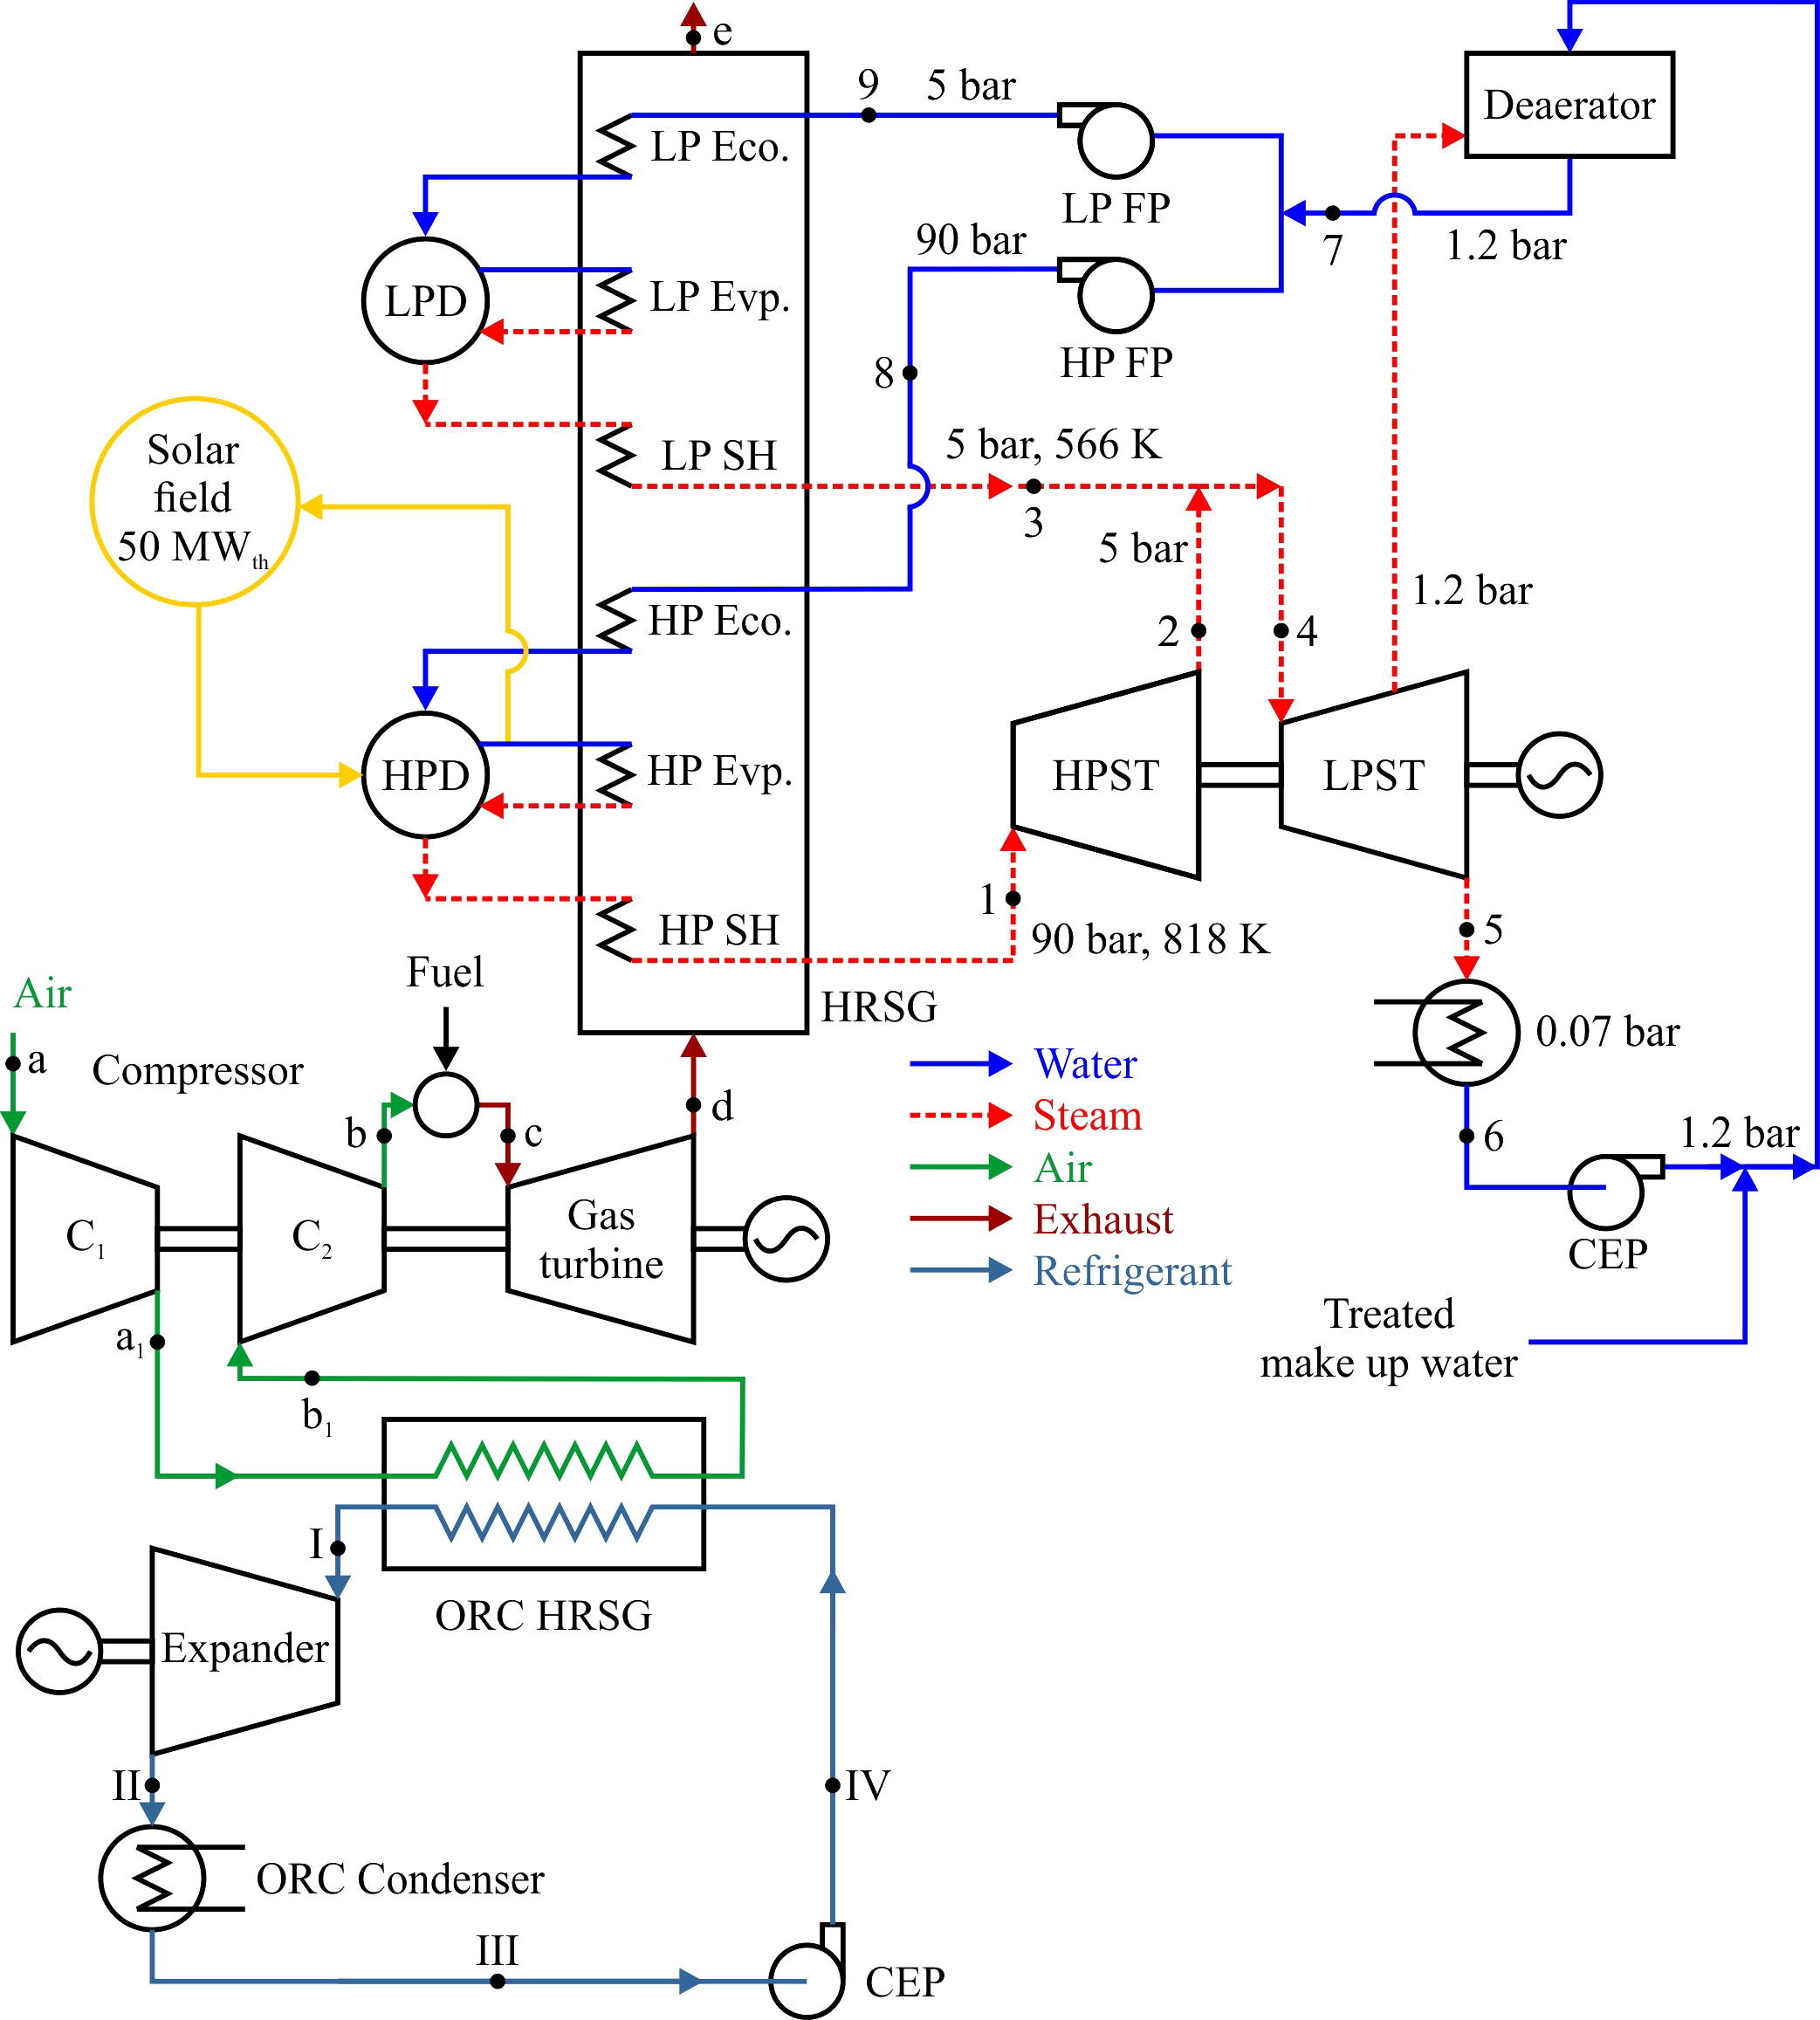
\includegraphics[width=.8\textwidth]{fig/Shaaban2016.jpg}
\caption{拥有两个底部循环的ISCC系统结构示意图}\label{fig:Shaaban2016}
\end{figure}

Alqahtani和Dalia\cite{Alqahtani2016}将ISCC电厂与独立CSP电厂、天然气联合循环电厂进行了对比分析。结果显示,将CSP整合进ISCC可以使发电成本比独立CSP电厂低35$\sim$40\%,并可以获得更好的调度能力。

Manente提出了一个具有三级压力的390$\,\mathrm{MWe}$的天然气联合循环来评估不同集成方案的ISCC。为了得到最高的年平均效率和太阳能份额,分别进行了增强输出功率和节约燃料的操作策略。结果显示,节约燃料的操作策略所获的年平均效率较低,这是因为燃气轮机的负荷下降导致系统整体效率下降。

Turchi等\cite{Turchi2014}提出了两种概念型的ISCC同槽式集热器混合设计的方案。在第一种方案中,燃气轮机的废气与在390$^\circ\mathrm{C}$以下运行的以导热油为传热流体的槽式集热器综合利用,在第二种方案中,燃气轮机的废气与在450$^\circ\mathrm{C}$以下运行的以熔融盐为传热流体的槽式集热器及蓄热系统(TES)一起综合利用。使用燃气轮机余热来补充TES系统为系统提供了操作灵活性,同时提高了天然气利用效率。

Mukhopadhyay和Ghosh~\cite{Mukhopadhyay2016}
提出了一种针对塔式太阳能电厂的热电联产梯级系统。该系统将传统燃气轮机的燃烧室用太阳能接收器替代,以布雷顿循环作为顶部循环。一个具有回热器的朗肯循环作为底部循环。

李晶等\cite{Li2016a}提出了一种新颖的梯级系统,该系统同时使用水工质朗肯循环和有机工质朗肯循环。水工质朗肯循环采用对两相流体适应性高的螺纹压缩机实现膨胀做功。水工质朗肯循环的凝结液用于驱动有机工质朗肯循环。

Al-Sulaiman\cite{AlSulaiman2014}分析了水工质-有机工质朗肯循环联合循环采用不同种类的有机工质所能获得的输出功率。在联合循环中,水工质朗肯循环由槽式集热器提供热量,有机工质朗肯循环由水工质朗肯循环的凝结热提供热量。结果表明,采用R134a的联合循环具有最佳㶲效率,其㶲效率可以达到26\%。

Dunham和Lipi\cite{Dunham2013}提出了组合布雷顿循环的分布式太阳能集热发电系统。通过对用于顶部布雷顿循环的工作流体和底部朗肯循环的工作流体进行分析后发现,使用二氧化碳的布雷顿顶部循环和使用R-245fa的朗肯循环底部循环的组合可以获得最高的组合循环效率,21.06%,而单独的二氧化碳布雷顿循环在相同的工况下仅可达到15.31%的峰值循环效率。

Bahrami等\cite{Bahrami2013}提出了一种联合有机工质朗肯循环。该朗肯循环用作斯特林循环的冷端散热器。有机工质循环的运行温度介于80$\mathrm{^\circ C}$到140$\mathrm{^\circ C}$之间。研究发现,联合循环的效率相比于独立的斯特林机可以提升4\%到8\%。

Thierry等\cite{Thierry2016}针对多级朗肯循环的两种不同结构提出了一种非线性优化方程。一种结构采用梯级利用的形式,一个循环作为顶部循环,另一个循环作为底部循环;另一种结构采用串联连接的形式让传热流体依次流经两个朗肯循环。经过对比分析发现,梯级结构可以获得比串联结构更高的效率,尤其是在热源温度较低的情况下。

Bahari等\cite{Bahari2016}考虑利用有机工质朗肯循环来回收利用斯特林机释放的热量。然而,该方案只是一个原始的设计,它没有考虑到应用于太阳能光热发电技术。

\nomenclature[C]{LFC}{Linear Fresnel Collector}

\section{文献综述小结}
通过对前人研究工作的总结可以发现,太阳能光热发电技术正迎来高速发展的黄金期。大量的研究人员从试验研究、机理模型、数学方法等方面对太阳能光热发电技术进行了相关研究。然而,他们多是针对现有太阳能光热技术进行改进性分析,也有文献提到了新的技术,比如空气槽式集热器、直接蒸汽生产系统等。但他们多是孤立的研究这些技术,没有把这些技术放进光热发电系统,尤其是梯级光热发电系统中进行研究。此外,也有少量文献研究太阳能的梯级收集或梯级利用。然而,没有文献针对太阳能光热梯级系统进行系统地分析,也没有文献梯级在一个梯级系统中同时能量的考虑梯级收集与梯级利用。

\section{研究内容}
\label{sec:researchContent}
% 改进点,重点,难度
% 技术路线

针对目前太阳能光热发电技术的特点,以及基于上述研究现状分析所存在的不足,本文以国家国际合作项目专项“太阳能梯级集热发电系统关键技术合作研究”为背景,目标是研究太阳能光热发电装置,利用各种传统型式的太阳能光热发电系统的优缺点以及热力特性,提出并组建、优化太阳能梯级集热发电系统,为探索出大规模低成本高效率利用太阳能的光热发电技术提供新的方案。主要研究内容包括:

\begin{enumerate}[label=(\arabic*)]
	
	\item 光热发电技术文献综述分析,对应于本文第一章。
	\setlength\parindent{2em}
	
	在简要介绍太阳能光热发电技术的研究背景及意义后,详细回顾了前人在已经商业应用的太阳能光热发电技术以及太阳能光热发电技术中的能量梯级收集利用领域所做的主要研究成果及研究现状,并简要概括了当前研究现状所存在的不足。
	\item 系统拓扑结构设计分析,对应于本文第二章。
	
	针对梯级系统拓扑结构的重要性及梯级发电系统结构选择的多样性,本文利用传统太阳能光热发电系统中各部件的特点,系统性地分析太阳能梯级发电系统的拓扑结构中的多种影响因素,提出多种采用梯级集热和梯级发电的太阳能光热梯级发电系统的拓扑结构方案。 

	\item 机理建模理论研究,对应于本文第三章。
	
	针对太阳能光热发电系统中关键部件的物理特性和运行机理,本文在关键部件的建模理论上进行深入研究。采用数学计算工具和系统开发工具,建立梯级系统中各部件的机理模型,进而组建梯级系统。采用面向对象的方法,充分利用封装、继承、多态等特性,保证各部件之间既具有独立性又具有关联性,同时保证系统中各模型易于替换和修改。最后开发了具有计算机软件著作权的太阳能光热发电开发系统。
	
	针对槽式集热器在长度方向上能量密度一致的特点,进行了整体换热系数沿长度方向均匀一致的假设,利用等热流密度下的流体与定温热源的传热计算公式,建立了槽式集热器的热效率计算模型。
	
	为碟式接收器建立了热网络模型,针对每一项热损失进行了详细地分析计算,通过求解热网络模型的各温度节点,得到碟式接收器的热效率计算模型。
	
	针对经典斯特林机模型考虑不可逆损失因素较少,计算误差较大的缺点,建立了考虑包括非理想换热、气体压力损失、活塞运动及摩擦损失、内部导热损失、穿梭导热损失等不可逆损失的斯特林机模型,并与经典模型和实验数据进行了对比分析。
	
	建立了\textbf{Stream}类用于部件的连接工作,部件的出口和入口用作连接的接口。两个不同的部件通过被赋值给同一个\textbf{Stream}对象而实现相互连接。以部件连接为基础实现了多部件间耦合计算功能。

	\item 斯特林机组排列方式优化研究,对应于本文第四章。
	
	考虑到斯特林机组不同排列方式对机组性能的影响,提出了五种基本的斯特林机组排列方式。利用太阳能光热开发系统建立了不同排列方式的斯特林机组仿真模型,并对其在不同影响因素下的性能进行了对比分析,找到了斯特林机组的最佳排列方式。

	\item 蒸汽发生系统的优化研究,对应于本文第五章。
	
	针对传统蒸汽发生系统在换热过程存在大量㶲损的缺点,本文提出了新型的分段加热系统,通过分段加热的方法来减少蒸汽发生过程中的温差,进而减少换热过程带来的㶲损,并降低太阳能场中传热流体的温度,提升太阳能光热系统的效率。
	
	在新型的分段加热系统中,太阳能场别分成三个片区,分别为预热过程、蒸发过程和过热过程供热。可以通过调整各片区传热流体的流量,降低其对应的换热温差,降低各片区的传热流体的温度,提升集热效率,并降低换热过程的㶲损,提升太阳能光热系统的效率。

	\item 梯级系统评估分析研究,对应于本文第六章。
	
	给出了梯级系统的性能评估指标——整体光电转换效率,并提出了合适的独立系统方案进行对比分析。通过选取合理的系统参数,利用太阳能光热发电开发系统对梯级系统和其对应的独立系统进行了建模仿真分析。分析了不同因素对梯级系统的效率提升的影响,并给出了有利于梯级系统实施的条件。

	\item 太阳能梯级发电实验台的建设及实验研究,对应于本文第七章。
	
	参与了太阳能梯级发电实验台的建设工作及实验研究。针对太阳辐射强度的不可控性、连续性及变化性,专门设计了特殊的实验工况来研究不同参数对槽式集热器和碟式集热器的集热效率的影响。设计了详细的实验步骤,明确了实验目的,并进行了相关的实验,获得了实验数据,并对建立的槽式集热器模型和碟式集热器模型进行了验证分析。
\end{enumerate}
\nomenclature[C]{CSP}{太阳能聚光集热发电}
%\nomenclature[C]{HTF}{传热流体}